\subsection{E6 --- Objection 1: the policy used the true attention for free}
\label{sec:est}
\textbf{Question.} E3--E5 fed the importance monitor the exact attention weight of every (token, layer) entry at every step. A real system must compute, approximate or sample this signal. How much of the saving survives an imperfect one? \textbf{Setup.} An \emph{estimator} sits between the true weights and the monitor (Fig.~\ref{fig:arch}); quality and access energy are still charged with the \emph{true} weights, so the policy simply acts on a worse signal. We test seven degradations on the 42 256M traces with dense reads, $10\times$ cost and the same leave-one-out protocol (thresholds re-selected per estimator over a 10-configuration grid; the oracle row reproduces E5):
\begin{itemize}[leftmargin=1.2em]
\item \emph{Noise} $\sigma\in\{0.25,0.5,1\}$: each weight is multiplied by an independent log-normal factor (for $\sigma{=}1$, a factor within $e^{\pm1}$ for 68\% of reads and mean-inflated by $1.65\times$).
\item \emph{Sampled}: the monitor sees attention only every 2nd, 4th or 8th step (EMA decay raised to the same power to keep its time constant).
\item \emph{Stale}: the monitor sees the weights from 1 or 4 steps ago.
\item \emph{Token-shared}: one score per token, the mean over layers, shared by all of its entries, i.e.\ what a system obtains if it can afford only one importance value per token rather than one per (token, layer).
\item Two combinations (token-shared with 4-step sampling; noise $\sigma{=}0.5$ with 4-step sampling).
\end{itemize}

\begin{figure}[t]
\centering
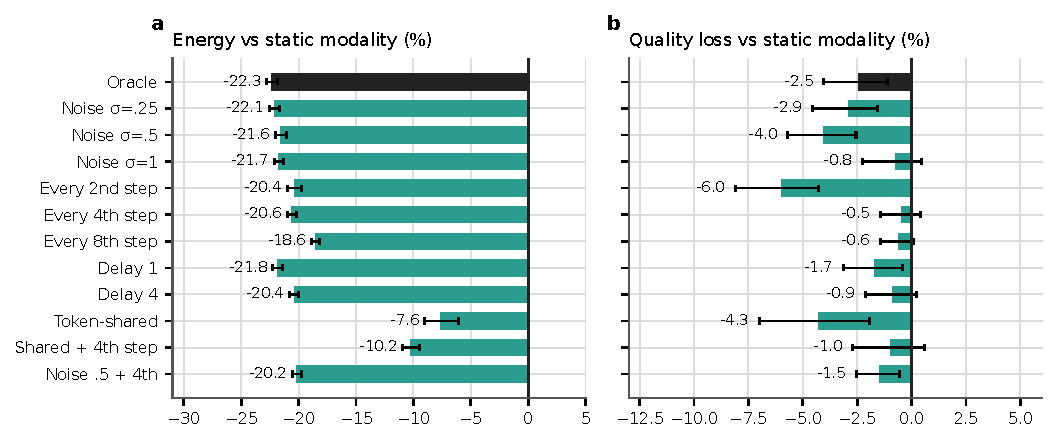
\includegraphics[width=0.93\linewidth]{figs/fig_estimators.pdf}
\caption{E6: held-out effect of the dynamic policy under imperfect importance signals (256M, 42 traces, dense reads, $10\times$; bars are leave-one-out means with bootstrap 95\% CIs; black = oracle). Per-entry signals can be noisy, sparse in time or stale and keep $\ge$18.6\% of the saving; a single score per token does not.}
\label{fig:est}
\end{figure}

\textbf{Finding 1: the saving is robust to a degraded per-entry signal.} Noise up to $\sigma{=}1$ leaves $-21.8\%$ energy (oracle $-22.3\%$); observing attention only every 8th step gives $-18.6\%$, a signal delayed by 4 steps gives $-20.4\%$, and noise plus 4-step sampling gives $-20.2\%$ (Fig.~\ref{fig:est}). All of these meet the pre-specified criterion (energy saving $\ge10\%$, quality change $\le+2\%$, CI excluding 0). Quality does not degrade: it stays at or below the static baseline (between $-6.0\%$ and $-0.5\%$), because a noisier or older signal promotes slightly more entries. The number of moves is essentially unchanged (1111--1298 against 1190 for the oracle). \textbf{Because the saving equals the energy a system may spend on estimation, the oracle's 22.3\% of static access energy is also the upper bound on the estimator's own cost per session}, and a signal sampled every 4th step still leaves $\sim$20\% of headroom.

\textbf{Finding 2: the signal must stay per (token, layer).} Collapsing importance to one score per token cuts the saving to $-7.6\%$ [$-9.0,-6.1$] (with 4-step sampling, $-10.2\%$), below the 10\% criterion. At the oracle's thresholds the token-shared signal reaches $-18.7\%$ energy but loses $+12.8\%$ quality, so the policy cannot find an operating point as good as the per-entry one. This is the same lesson as E4, seen from the signal side: what the policy exploits is variation \emph{between layers of the same token}, not a per-token summary. \textbf{Caveat.} All estimators here are free; we charge no energy or latency for producing them, and do not model any specific approximate scorer (e.g.\ low-precision or sampled key scores). E6 shows how imperfect the signal may be, not what a concrete estimator costs.
